\documentclass[../../main.tex]{subfiles}
\begin{document}

{\bf [解]}
$(t,e^t)$ における $y=e^x$ の接線 $\ell_t$ は，$(e^x)'=e^x$ より，
\begin{align}
\ell_t: y=e^t(x-t)+e^t \label{eq:1}
\end{align}
である．これが $(a,b)$ を通る時，
\begin{align}
b=e^t(a-t)+e^t\equiv f(t) \label{eq:2}
\end{align}
を満たす．

\begin{figure}[htb]
\centering
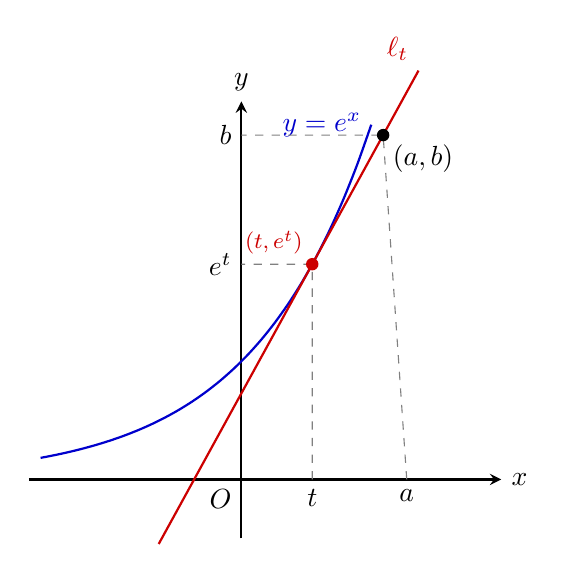
\begin{tikzpicture}[scale=1.5, >=stealth]
  % 座標軸
  \draw[->, thick] (-1.8, 0) -- (2.2, 0) node[right] {$x$};
  \draw[->, thick] (0, -0.5) -- (0, 3.2) node[above] {$y$};
  \node[below left] at (0,0) {$\text{O}$};

  % y = e^x の曲線
  \draw[domain=-1.7:1.1, smooth, thick, blue!80!black] plot (\x, {exp(\x)}) node[left] {$y=e^x$};

  % 接点 (t, e^t) --- 例として t = 0.6
  \coordinate (P) at (0.6, 1.822);
  % 外部の点 (a, b) --- b = e^0.6 * (1.2 - 0.6 + 1) = 1.6 * 1.822 = 2.915
  \coordinate (AB) at (1.2, 2.915);

  % 接線 l_t : y = e^t(x - t) + e^t
  \draw[thick, red!80!black, domain=-0.7:1.5] plot (\x, {1.822*(\x - 0.6) + 1.822}) node[above left] {$\ell_t$};

  % 点 (a,b) からのガイド線
  \draw[dashed, gray] (1.4, 0) -- (AB) -- (0, 2.915);
  \node[below] at (1.4, 0) {$a$};
  \node[left] at (0, 2.915) {$b$};

  % 接点 (t, e^t) からのガイド線
  \draw[dashed, gray] (0.6, 0) -- (P) -- (0, 1.822);
  \node[below] at (0.6, 0) {$t$};
  \node[left] at (0, 1.822) {$e^t$};

  % プロット点
  \fill[red!80!black] (P) circle (1.5pt) node[above left, font=\footnotesize] {$(t, e^t)$};
  \fill[black] (AB) circle (1.5pt) node[below right] {$(a,b)$};
\end{tikzpicture}
\caption{$y=e^x$ と $(a,b)$ を通る接線 $\ell_t$}
\end{figure}

$y=e^x$ では，接点が異なれば接線が異なるので，\cref{eq:2}をみたす $t$ の数が $(a,b)$ から引きうる接線の数に等しい．
そこで$f(t)$の挙動を調べるため一階微分を計算すると
\begin{align}
f'(t)=e^t(a+1-t-1)=e^t(a-t)
\end{align}
から，増減表は以下のようになる．

\begin{table}[htb]
 \begin{center}
\caption{$f(t)$の増減表}
\begin{tabular}{c|ccccc}
$t$ & $-\infty$ & $\dots$ & $a$ & $\dots$ & $\infty$ \\
\hline
$f'$ & & $+$ & $0$ & $-$ & \\
\hline
$f$ & $(0)$ & $\nearrow$ & $e^a$ & $\searrow$ & $(-\infty)$
\end{tabular}
\end{center}
\end{table}

よって$y=f(t)$ のグラフは下図のようになる．

\begin{figure}[htb]
\begin{center}
\begin{tikzpicture}[scale=1.9, >=stealth]
  % 座標軸
  \draw[->] (-1.6,0) -- (1.9,0) node[right] {$t$};
  \draw[->] (0,-0.9) -- (0,1.7) node[above] {$y$};
  % y=f(t)=e^t(a+1-t) のグラフ (a=0.4 として図示。t=a で最大値e^a, t=a+1で0)
  \draw[domain=-1.4:1.53, smooth, thick] plot (\x, {(1.4-\x)*exp(\x)});
  \draw[dashed] (0.4,0) -- (0.4,1.4918);
  \draw[dashed] (0,1.4918) -- (0.4,1.4918);
  \fill (0.4,1.4918) circle (0.63pt);
  \node[left] at (0,1.4918) {$e^a$};
  \node[below] at (0.4,0) {$a$};
  \node[below] at (1.4,0) {$a+1$};
\end{tikzpicture}
\end{center}
\caption{$y=f(t)$のグラフの概形}
\end{figure}

したがって $a$ を固定した時，\cref{eq:2} $y=b$，$y=f(t)$ の二つのグラフの交点で与えられるので求める解の個数は

\begin{align}
\begin{cases}\displaystyle
b\le0\ \text{の時，解は}1\text{つ} \\
0<b<e^a\ \text{の時，}2\text{つ} \\
b=e^a\ \text{の時，}1\text{つ} \\
b>e^a\ \text{の時，}0\text{個}
\end{cases}
\end{align}
となる．$a$ の固定を解除して整理すると
\begin{align}
\begin{cases}\displaystyle
b\le0\ \text{または}\ b=e^a\ \text{の時}\quad 1\text{個} \\
0<b<e^a\ \text{の時}\quad 2\text{個} \\
b>e^a\ \text{の時}\quad 0\text{個}
\end{cases}
\end{align}
が求める解の個数である．

\begin{figure}[htb]
\centering
\begin{tikzpicture}[scale=1.5, >=stealth]
  % 領域の塗り分け
  % 1. 0個の領域 (b > e^a)
  \fill[red!15] (-2.2, 0) -- plot[domain=-2.2:1.0] (\x, {exp(\x)}) -- (1.0, 2.7) -- (-2.2, 2.7) -- cycle;

  % 2. 2個の領域 (0 < b < e^a)
  \fill[blue!15] (-2.2, 0) -- plot[domain=-2.2:1.0] (\x, {exp(\x)}) -- (1.0, 0) -- cycle;

  % 3. 1個の領域 (b <= 0)
  \fill[gray!20] (-2.2, 0) rectangle (2.0, -1.0);

  % 軸描画
  \draw[->, thick] (-2.2, 0) -- (2.2, 0) node[right] {$a$};
  \draw[->, thick] (0, -1.0) -- (0, 2.8) node[above] {$b$};
  \node[below left] at (0,0) {$\text{O}$};

  % b = e^a の曲線
  \draw[domain=-2.2:1.0, smooth, very thick, blue!80!black] plot (\x, {exp(\x)});
  \node[above left, blue!80!black] at (-1.0, 0.368) {$b=e^a$};

  % b = 0 (a軸) の強調
  \draw[very thick, black] (-2.2, 0) -- (2.0, 0);

  % 各領域の解の個数テキスト
  \node[font=\small\bfseries, red!70!black] at (-0.8, 1.8) {$0$ 個 ($b > e^a$)};
  \node[font=\small\bfseries, blue!80!black] at (0.7, 0.5) {$2$ 個 ($0 < b < e^a$)};
  \node[font=\small\bfseries, black!70] at (0.5, -0.5) {$1$ 個 ($b \le 0$)};
  \node[font=\small\bfseries, blue!80!black, align=center] at (-1.5, -0.6) {境界上の $b=e^a$\\も $1$ 個};

\end{tikzpicture}
\caption{$ab$ 平面における接線の本数（解の個数）の領域}
\end{figure}


\newpage

\end{document}
